
\label{sec:model}

\textcolor{red}
{O problema de roteamento de caminhões betoneira consiste em um conjunto de clientes que precisam de receber uma determinada quantidade de concreto em suas instalações. Para atender a essa demanda, são realizadas uma ou mais viagens cujos instantes de entregas devem ocorrer dentro de janelas de um dado horizonte de tempo. O concreto é provido por um conjunto de plantas com capacidade de fornecimento de concreto limitada e é entregue por uma frota de veículos de capacidades homogêneas que são distribuídos entre as plantas no início do horizonte de tempo. Os caminhões atribuídos a cada planta ficam vinculados à mesma  até o fim de cada horizonte de tempo de trabalho. Os caminhões atendem somente a um cliente por viagem e podem realizar várias viagens para diversos clientes, respeitadas as suas capacidades e o tempo de viagem entre as plantas e os canteiros de obras.}

Algumas das características do problema são que os clientes tendem a ser atendidos pelas plantas mais próximas, mas ser atendido por uma planta mais distante pode facilitar novos arranjos gerais; a atribuição de viagens para os clientes em uma ordem aleatória baseia uma solução, contando que sejam respeitadas as restrições de capacidade dos veículos e das plantas; num caso de apenas um veículo, priorizar um cliente mais caro cujo tempo de entrega não colide com outros é mais viável que priorizar um mais barato que colide com outros dois; mudar a ordem de apenas um cliente possibilita alterar sua influência sobre a solução e facilita identificar toda a sequência de eventos advindas dessa mudança; mudar a ordem de todos os clientes possibilita disrupções das soluções (saída do ótimo local), porém dificulta a identificação da sucessão de eventos de cada alteração individual; não é necessário atribuir os veículos aos clientes para saber se os veículos serão capazes de atender todos os clientes; basta conferir se, ao alocar as viagens dos clientes às plantas, ignorando os veículos, a quantidade de clientes atribuídos à planta em cada instante de tempo é menor ou igual à quantidade de veículos disponíveis para essa mesma planta.

A seguir temos a descrição de todas as variáveis e parâmetros utilizados no modelo, seguidos pelo modelo. 


\begin{table}[h!]
  \centering
  \begin{tabular}{cl}
  \toprule
  \textbf{Parâmetro} & \textbf{Descrição} \\
  \hline
  I & Conjunto de plantas $I=\{1,\ldots,n_i\}$\\
  J & Conjunto de clientes, $J = \{1,\ldots,n_j\}$ \\
  K & Conjunto de veículos disponíveis $K=\{1,\ldots,n_k\}$\\
  L & Conjunto de viagens possíveis $L=\{1,\ldots,n_l\}$\\
  $c_{ij}$ & custo do atendimento do cliente $j\in J$ pela planta $i\in I$ \\
  q & capacidade dos caminhões \\
  q$_{i}$ & capacidade das plantas \\
  $d_{j}$ & demanda total do cliente j \\
  $t_{ij}$ & tempo que qualquer caminhão demora para ir da planta i ao cliente j \\
  $t_{ji}$ & tempo que qualquer caminhão demora para ir do cliente j à planta i \\
  $a_{j}$ & tempo de abertura da janela de entrega do cliente j \\
  $b_{j}$ & tempo de abertura da janela de entrega do cliente j\\
  $T$ & horizonte de tempo de um dia de trabalho \\
  \hline
  \end{tabular}
  \caption{Lista de Parâmetros}
  \label{tab:parametros}
\end{table}


\begin{table}[ht!]
  \centering
  \begin{tabular}{p{3cm}p{10cm}}
  \toprule
  \textbf{Variáveis} & \multicolumn{1}{c}{\textbf{Descrição}} \\
  \midrule
  $x_{ijlr}\in \{0,1\}$ & variável binária que, quando ativa, indica que o veículo $k \in K$, em sua l-é\-si\-ma via\-gem $l\in L_k$, sai
  da planta $i\in I$ para o cliente $j\in J$ \\
  u$_{ik}$ & variável binária que, quando ativa, indica que o veículo k está atribuído à planta i \\
  s$_{kl}\geq 0$ & momento de início da l-ésima viagem do veículo k \\
  \bottomrule
  \end{tabular}
  \caption{Lista de Variáveis}
  \label{tab:variables}
\end{table}



\begin{align}
\label{eq1: obj} \min & \sum_{i \in I} \sum_{j \in J} \sum_{l \in L} \sum_{r \in R} c_{ij} \cdot x_{ijlr} + \sum_{i \in I} vehic\_cost \cdot z_i \\
\text{sujeito a: }
\label{eq2: demand} & \sum_{i \in I} \sum_{r \in R} x_{ijlr} = 1, \quad \forall j \in J, \forall l \in L[j] \\
\label{eq3: capacity} & \sum_{j \in J}\sum_{l \in L[j]} \sum_{r \in R} d_{jl} \cdot x_{ijlr} \leq q_i, \quad \forall i \in I, \forall l \in L[j] \\
\label{eq4: trucks} & \sum_{j \in J} \sum_{r \in R} x_{ijlr} \leq z_i, \quad \forall r \in T, \forall i \in I, \forall l \in L[j] \\
% \label{eq5: total_trucks} & \sum_{i \in I} z_i \leq md\_static\_TW\_cost[2] \\
% \label{eq6: total_cost} & \sum_{i \in I} \sum_{j \in J} \sum_{l \in L} \sum_{r \in R} cost_{ij} \cdot x_{ijlr} + \sum_{i \in I} vehic\_cost \cdot z_i \leq md\_static\_TW\_cost[0] \\
\label{eq7: binary_x} & x_{ijlr} \in \{0, 1\}, \quad \forall (i, j, l, r) \in I \times J \times L \times R \\
% \label{eq8: binary_z} & z_i \in \{0, 1\}, \quad \forall i \in I
\end{align}

\textcolor{red}{Onde a função objetivo é reduzir o custo do transporte associado ao somatório das l viagens dos clientes j  com origem nas plantas i e início nos instantes r, mais o somatório do custo de alocação dos veículos utilizados. A restrição um estabelece que todo cliente, em cada uma de suas viagens, deve ser atendido por uma única planta i e ter um único instante de início r. A restrição dois estabelece que a capacidade q$_i$ de cada planta deve ser maior ou igual ao somatório de toda demanda d$_{jl}$ atribuída a essa planta. }
% A restrição 4 estabelece que o total de veículos utilizados deve ser inferior ao total de veículos disponíveis.
\subsection*{Instâncias}
\label{sec:instcomp}

% Outro fator simplificado diz respeito à carga, que antes heterogênea passou a ser homogênea. Esse fator pode resultar em discrepâncias dos resultados finais, ainda que haja no Brasil uma concentração de veículos com a capacidade de 8m³.

As faixas dos recursos das instâncias criadas são determinadas aleatoriamente baseando-se nas informações disponíveis sobre as instâncias do trabalho de \cite{cantu}. Além de nos basearmos nessas informações, realizamos alterações relacionadas com a quantidade de veículos para que as execuções das soluções não tenham folga excessiva dos recursos. Dados relacionados à demanda dos clientes e às capacidades das plantas foram estabelecidos de forma empírica.

Segue um conjunto de postulados para o presente trabalho: item a abertura da janela de tempo de cada cliente deve ser maior ou igual ao tempo da viagem mais demorado das plantas para esse mesmo cliente; o fechamento da janela de tempo deve inferior ao tempo máximo da última entrega mais a maior viagem;a velocidade média dos veículos é de 40 km/k; um dia de serviço tem 600 minutos; cada entrega tem um período de tempo de 20 minutos para ser realizada e não colide com as demais entregas de um mesmo cliente; a capacidade de carga de todos os caminhões é de 8m³ por viagem;a demanda de cada cliente foi aleatória entre 3 e 30m³; a capacidade de cada planta foi aleatória entre 1/quantidade de plantas + aleatório entre 0 e 50\% da demanda total; as coordenadas geográficas x e y de todas as plantas e todos os clientes assumiram valores aleatórios entre 0 e 30 km; o custo de atendimento de um cliente é, a princípio, igual à distância do mesmo até as plantas; o custo de não atendimento de um cliente é equivalente a duas vezes o custo do cliente mais caro da instância; o tempo de descarregamento é nulo.

% Nota-se que, como \cite{cantu} não esclarece a demanda média por cliente,  não é possível avaliar o nível de demanda dos recursos para replicar de forma fidedigna, mas partindo do pressuposto de que seus clientes seguiam médias como as estabelecidas ṕor \cite{XXXXXXXXXXXXXXXXXXXX} ou \cite{XXXXXXXXXXXXXXXXXXXX}, há sobra de recursos para todas as instâncias de teste do modelo.

Foram gerados dois grupos de instâncias divididos entre 3 ou 5 plantas. Para cada grupo a quantidade de clientes foi alternada de 5 em 5 para um total de entre 10 e 50 clientes. A geração dos limites superiores foi dada seguindo as etapas: 1º - estabelece-se se a quantidade de plantas e clientes disponíveis; realiza-se a heurística construtiva gananciosa considerando caminhões betoneira ilimitados; reduz-se de um em um a quantidade de caminhões até que a heurística greedy retorne inviabilidade; retorna a última instância cujo método ganancioso obteve sucesso; calcula-se o custo da instância recebida.

Os dados do postulado servem para nortear a reprodução, porém não são precisam ser estáticos. Foram consideradas as distâncias linear entre as plantas e os clientes. Abaixo segue uma instância do problema, onde cada cliente pode ter mais de uma viagem atrelada:

\begin{figure}[H]
  \centering
  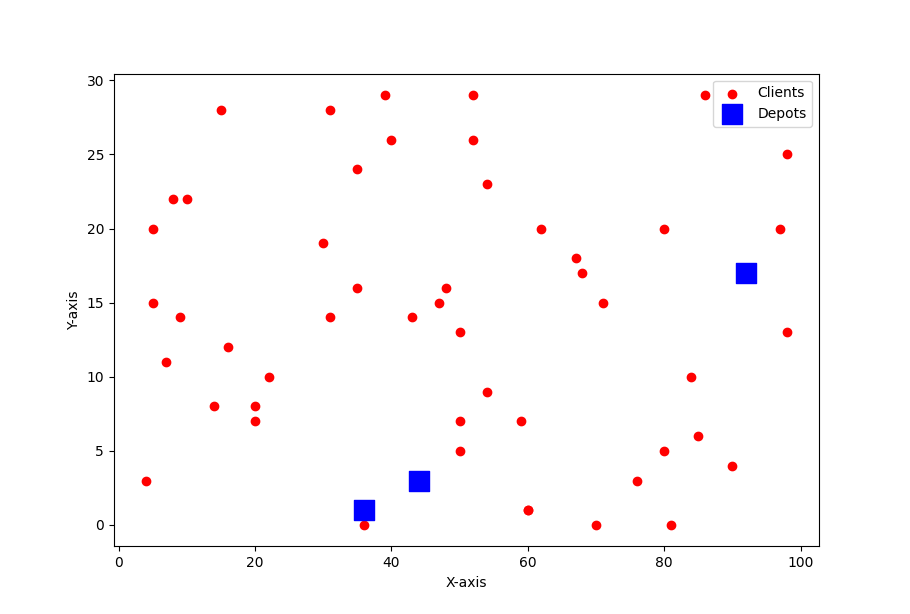
\includegraphics[width=\linewidth]{img/inst_1.png}
  \caption{Instância do problema}
  \label{fig:inst1}
\end{figure}

\subsection*{Estrutura de dados}
\label{subsec:estruturadosdados}
\textcolor{red}{A principal estrutura de dados utilizada nas heurísticas e nos modelos é dedicada à representação das plantas, onde podemos acessar em cada instante as viagens que são realizadas. Mais profundamente, corresponde a um vetor de tamanho igual ao horizonte de tempo, onde cada posição desse vetor armazenará as viagens que ocorrerão em cada um dos seus instantes. Por exemplo, caso a viagem 3 seja executada no período de 10 a 20, adicionaremos o valor 3 nas posições [10,20) do vetor. A quantidade de viagens em cada instante representa a quantidade mínima de veículos utilizadas por essa planta nesse instante. A maior quantidade de viagens simultâneas representará a quantidade de veículos utilizados pela planta. 
Na imagem abaixo, vemos uma representação dessa estrutura de dados utilizada.}

% \captionsetup{aboveskip=0pt,belowskip=1pt}
\begin{figure}[H] % "H" ensures the figure stays in the exact place
  \centering
  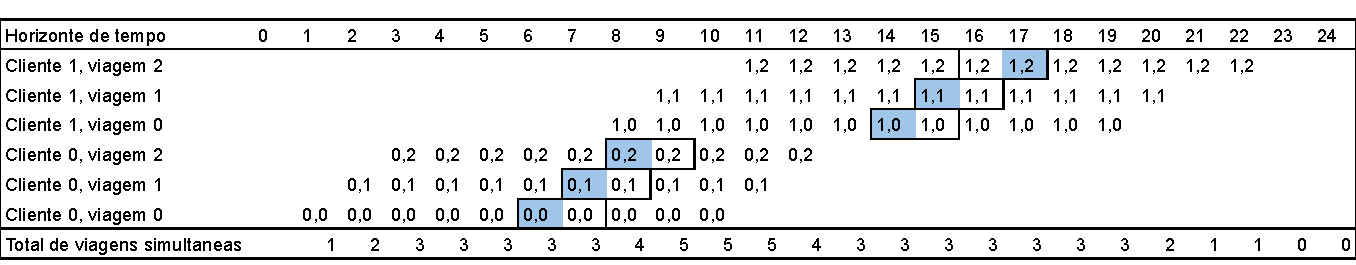
\includegraphics[width=1\textwidth]{img/estrutura de dados.pdf}
  \caption{Estrutura de Dados}
\end{figure}

 \textcolor{red}{No exemplo da figura acima, temos a atribuição das viagens de dois clientes a uma planta. A janela de tempo para entrega é de duas unidades de tempo e estão com bordas nos instantes cuja entregas são permitidas. As viagens do cliente 0 custam 4 unidades de tempo para a ida e 4 unidades de tempo para a volta, enquanto as viagens do cliente 1 custam 6 unidades de tempo em cada sentido. Os instantes em azul indicam o momento das entregas.
Nesse exemplo, a viagem 2 do cliente 1 foi executada no último instante da janela de tempo, fazendo assim com que a quantidade de viagens simultâneas no instante 10 não chegasse a seis, fazendo com que a necessidade de veículos nessa planta não superasse 5 em nenhum instante. }